% Compile with: pdflatex poissongam_beamer.tex
% Figures must be in beamer_figures/ (extracted from notebook)

\documentclass{beamer}
\usetheme{Madrid}
\usecolortheme{default}
\usepackage{graphicx}
\usepackage{amsmath}
\usepackage{listings}
\usepackage{xcolor}

\lstset{
  basicstyle=\ttfamily\small,
  breaklines=true,
  frame=single,
  backgroundcolor=\color{gray!10}
}

\title{PoissonGAM for Precipitation Modeling}
\author{Educational Notebook}
\institute{}
\date{}

\begin{document}

\frame{\titlepage}

\begin{frame}{Overview}
  \begin{itemize}
    \item Poisson GAMs for wet-day count data
    \item \textbf{Poisson}: count data with mean $\approx$ variance
    \item \textbf{Log link}: $\log(\mu) = f(x) \Rightarrow \mu = \exp(f(x))$
    \item Use when: counts, many zeros, mean $\approx$ var
    \item Avoid for: continuous outcomes, overdispersion (NegativeBinomialGAM), binary (LogisticGAM)
  \end{itemize}
\end{frame}

\begin{frame}{Exploratory Data: Distribution and Seasonality}
  \begin{itemize}
    \item \textbf{Left:} Histogram of non-zero precipitation amounts (log scale). Right-skewed, many small values---typical for precipitation.
    \item \textbf{Right:} Daily precipitation for one sample year across day of year, showing seasonal variation.
  \end{itemize}
  \begin{center}
    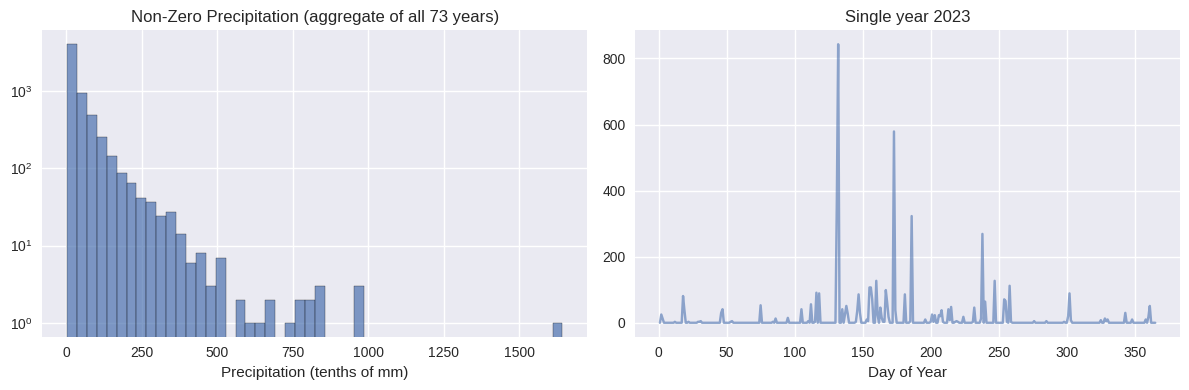
\includegraphics[width=0.85\textwidth]{beamer_figures/fig_01.png}
  \end{center}
\end{frame}

\begin{frame}{Data Prep: Wet-Day Counts per Period}
  \begin{itemize}
    \item Model wet-day counts (not amounts) per 2-week period
    \item Check variance $\approx$ mean before fitting Poisson
    \item Period length = 14 days
  \end{itemize}
  \begin{block}{Key idea}
    Count of wet days per period is a true Poisson process: ``How many wet days occur in this period?''
  \end{block}
\end{frame}

\begin{frame}[fragile]{Fit PoissonGAM per Year}
  \begin{itemize}
    \item $s(0)$ = smooth spline on day of year
    \item \texttt{n\_splines=12}, \texttt{spline\_order=3}
    \item Separate model per year for year-specific seasonal patterns
    \item \texttt{gridsearch} tunes the smoothing penalty $\lambda$ (reported in the notebook)
  \end{itemize}
  \begin{exampleblock}{Code (sparingly)}
\begin{lstlisting}
# Build the model (structure) first...
gam = PoissonGAM(s(0, n_splines=12, spline_order=3))

# ...then tune the smoothing penalty lambda via CV grid search
gam = gam.gridsearch(X, y)

# Selected smoothing strength (lambda) used for this fit:
print("selected lambda =", gam.lam)
\end{lstlisting}
  \end{exampleblock}
\end{frame}

\begin{frame}{Observed vs Fitted: Single Year (2023)}
  \begin{itemize}
    \item Points = observed wet-day counts per 2-week period
    \item Blue curve = PoissonGAM spline fit
    \item Shaded band = 95\% prediction interval
    \item Peaks and troughs show seasonal wetness
  \end{itemize}
  \begin{center}
    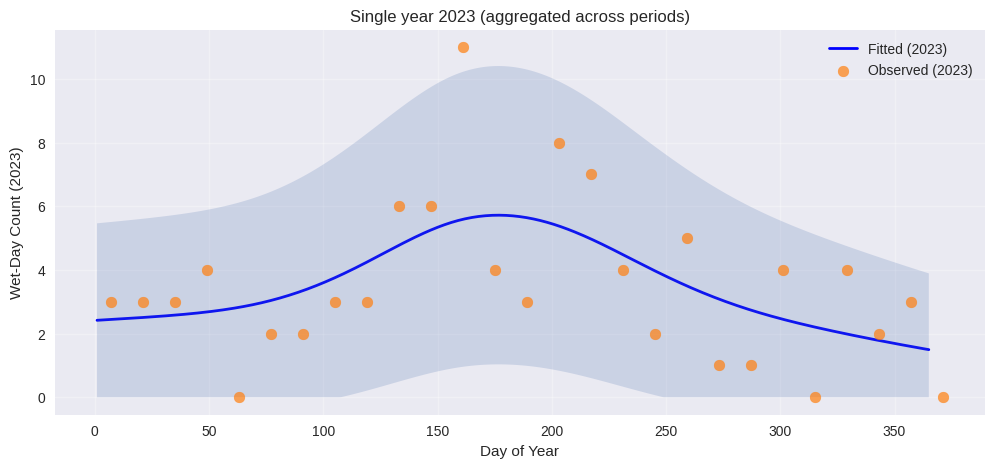
\includegraphics[width=0.75\textwidth]{beamer_figures/fig_02.png}
    
    \vspace{1mm}
    \scriptsize Selected smoothing $\lambda$ (CV \texttt{gridsearch}): \texttt{[[63.0957344480193]]}
  \end{center}
\end{frame}

\begin{frame}{Observed vs Fitted: Multiple Years}
  \begin{columns}
    \column{0.5\textwidth}
    \textbf{2013--2023 aggregate}\\
    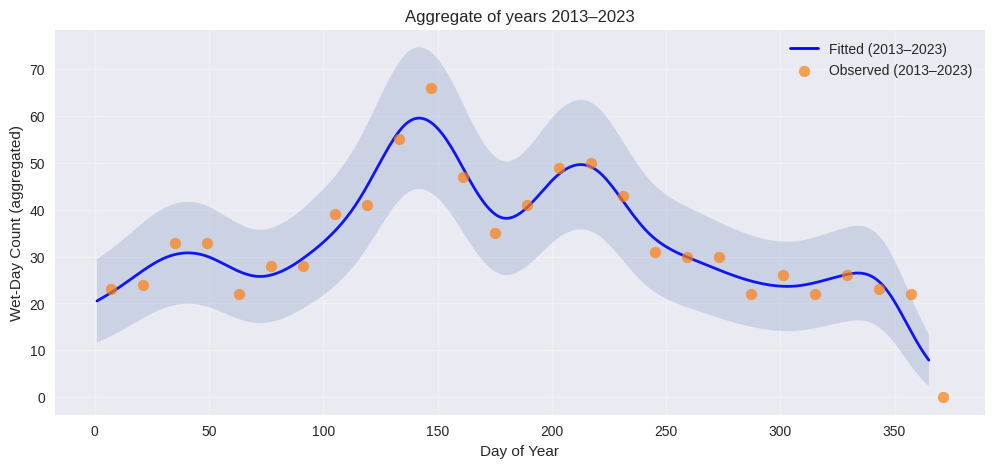
\includegraphics[width=\textwidth]{beamer_figures/fig_03.png}
    
    \vspace{1mm}
    \scriptsize Selected smoothing $\lambda$: \texttt{[[1.0]]}
    \column{0.5\textwidth}
    \textbf{All years aggregate}\\
    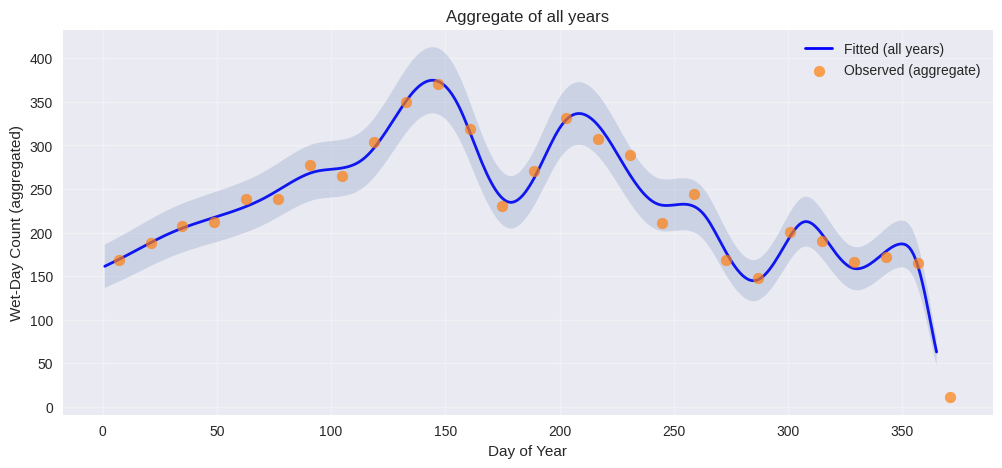
\includegraphics[width=\textwidth]{beamer_figures/fig_04.png}
    
    \vspace{1mm}
    \scriptsize Selected smoothing $\lambda$: \texttt{[[0.015848931924611134]]}
  \end{columns}
\end{frame}

\begin{frame}{Why Deviance Residuals Instead of Raw?}
  For Poisson, raw residuals $r = y - \mu$ are not ideal:
  \begin{itemize}
    \item \textbf{Heteroscedasticity}: $\mathrm{Var}(Y) = \mu$, so variance of $r$ changes with $\mu$
    \item \textbf{Q-Q plots}: Raw residuals don't approximate normality well
    \item \textbf{Comparability}: Residuals at different fitted values aren't on a common scale
  \end{itemize}
  We use \textbf{deviance residuals} instead.
\end{frame}

\begin{frame}{Deviance Residual Formula}
  \[
  d_i = \mathrm{sign}(y_i - \mu_i) \cdot \sqrt{2 \left[ y_i \log(y_i/\mu_i) - (y_i - \mu_i) \right]}
  \]
  \vspace{0.5em}
  Signed square-root of each observation's contribution to the deviance. For Poisson, deviance residuals have approximately constant variance and are closer to normal.
\end{frame}

\begin{frame}{Raw vs Deviance Residuals}
  \begin{center}
    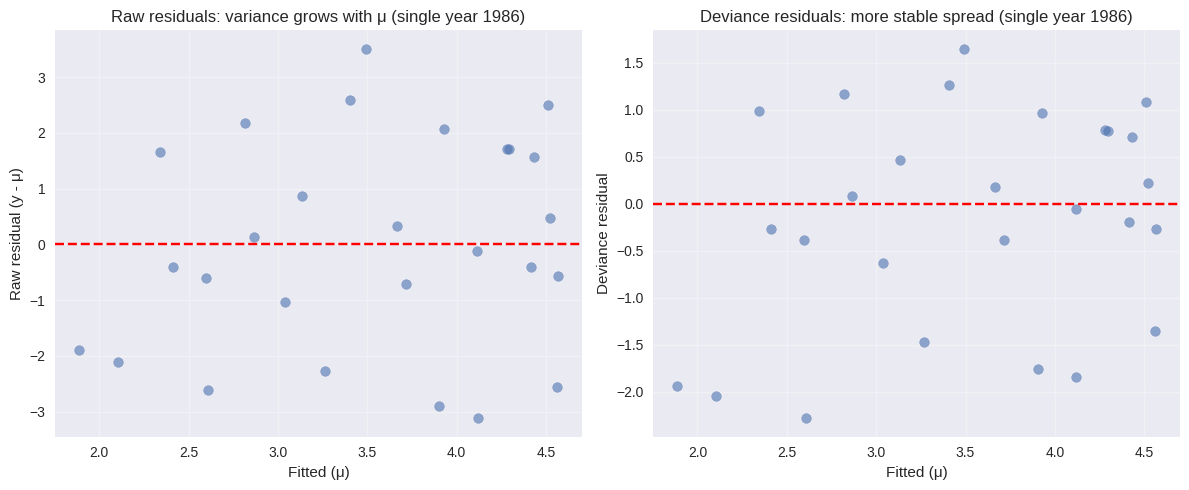
\includegraphics[width=0.9\textwidth]{beamer_figures/fig_05.png}
  \end{center}
  \small Left: variance grows with $\mu$. Right: more stable spread.
\end{frame}

\begin{frame}{Model Diagnostics}
  \begin{itemize}
    \item \textbf{Top-left:} Residuals vs fitted---points roughly around zero
    \item \textbf{Top-right:} Q-Q plot---deviation from red line common for Poisson
    \item \textbf{Bottom-left:} Observed vs predicted for one year
    \item \textbf{Bottom-right:} Fitted curve with 95\% prediction interval
  \end{itemize}
  \begin{center}
    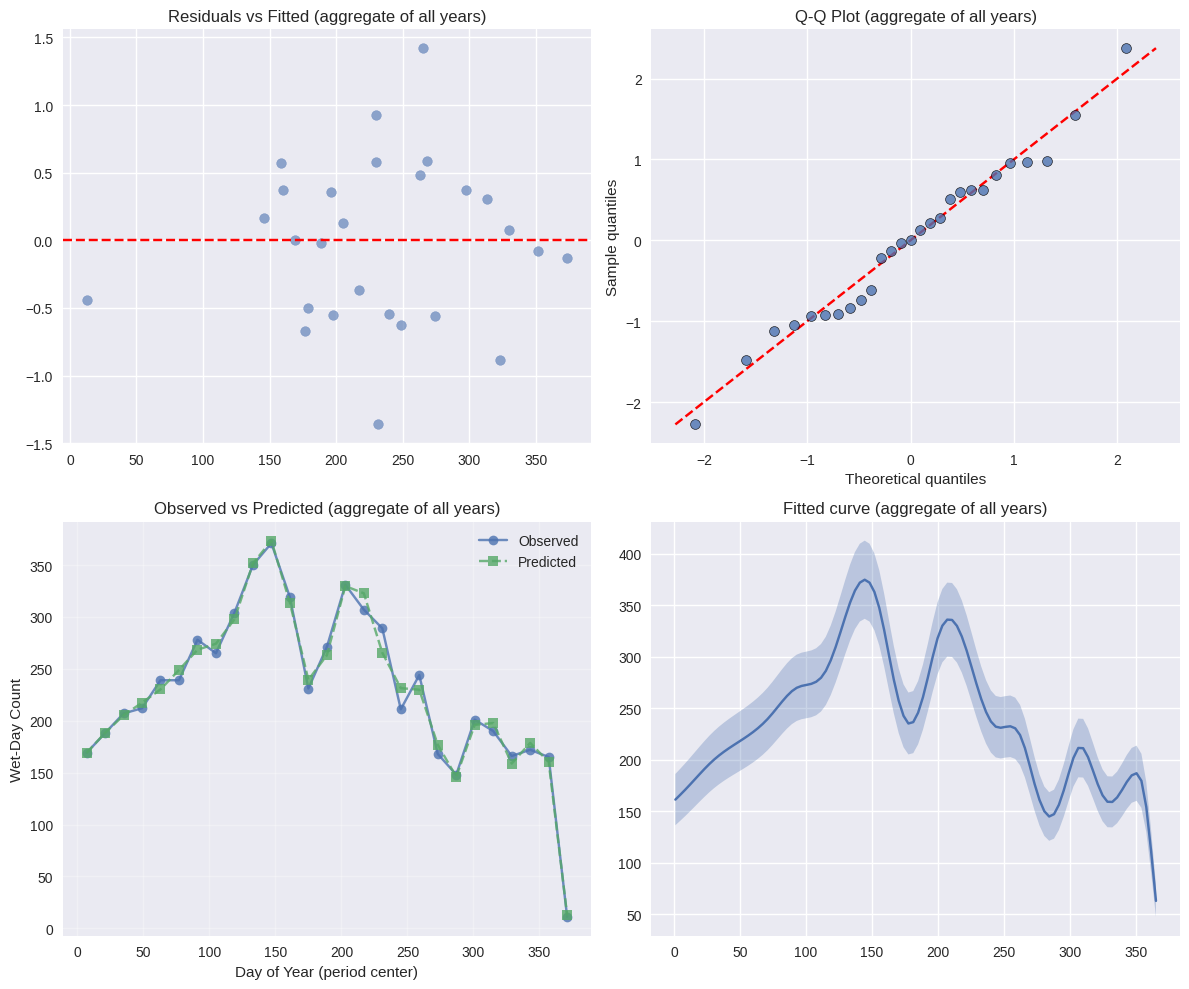
\includegraphics[width=0.7\textwidth]{beamer_figures/fig_06.png}
  \end{center}
\end{frame}

\begin{frame}{Interpretation}
  \begin{itemize}
    \item \textbf{Log link}: $\log(\mu) = f(\mathrm{day}) \Rightarrow \mu = \exp(f)$. Peaks = wetter periods.
    \item \textbf{When to use PoissonGAM}: count data, mean $\approx$ var
    \item \textbf{Alternatives:}
    \begin{itemize}
      \item NegativeBinomialGAM (overdispersion)
      \item GammaGAM (amounts)
      \item LogisticGAM (binary)
    \end{itemize}
  \end{itemize}
\end{frame}

\begin{frame}{Summary}
  \begin{enumerate}
    \item PoissonGAM captures smooth seasonal patterns in wet-day counts
    \item Log link ensures positive predictions
    \item Spline terms model non-linear relationships
    \item Deviance residuals preferred over raw for diagnostics
    \item Year-level totals can match well even if individual 2-week periods are noisy: errors can cancel when you sum/average over the whole year
  \end{enumerate}
\end{frame}

\end{document}
